% siminos/kittens/catlatt.tex      pdflatex CL18
% $Author: predrag $ $Date: 2020-09-05 23:05:02 -0500 (Sat, 05 Sep 2020) $

\section{\catLatt} % {Herding cats}  %
\label{s:catlatt}


The \emph{\templatt} of \refsect{s:kickRot}  is a 1\dmn\ example of the simplest
{\spt}ly chaotic, or `turbulent' field theory, the {\em \catlatt} to
which we turn now. \catLatt\ lives on a  $d$\dmn\ discretized spacetime,
a {\spt} $\integers^d$ integer lattice, with a cat map (a `rotor') on
each site, coupled to its nearest neighbors. Another way of visualizing a
\catlatt\ is as a lattice of locally hyperbolic `anti' oscillators, as
opposed to the classical free field theory, with an oscillator at each
site.
        \PC{2020-02-23} {
Probably need to refer to the Gaussian model here - see Kadanoff.
        }

The \templatt\ lives on a $1$\dmn\ temporal integer lattice $\integers$,
with very  simple `tilings'. For every integer temporal period
$\period{}$, we first determine $N_\period{}$, the number of all periodic
\emph{lattice state} ${\Xx}_{\Mm}$ solutions on a tile of length
$\period{}$. However, if $\period{}=m\period{p}$, the $\period{}$-tile
can be tiled by $m$ repeats of a smaller  $\period{p}$-tile, so {some} of
$\period{}$-{\po} {solutions} are repeats of the already determined
shorter $\period{p}$ \emph{prime} solution  $\Xx_p$. Furthermore, due to
the time invariance of the defining equations, there are $\period{p}$
physically equivalent copies of a given solution in the time orbit of
every $\Xx_p$. So all we really have to do is to enumerate $M_\period{}$
{\em prime orbits} of the time-invariance equivalent \po\ solutions,
whose generating function is the analytically elegant {\tzeta}.

For the $d$\dmn\ \catlatt\ the repertoire of periodic tilings is richer.
In $d=2$ and $3$ the basic facts are well known both from
crystallography, and from the number theory of integer lattices. In this
paper we systematically construct and enumerate distinct $d=2$ tilings,
or Bravais lattices $\LTS{}{}{}$, of increasing spacetime periodicities,
and determine $N_{\LTS{}{}{}}$, the number of \emph{doubly periodic
lattice state} solutions, by evaluating the associated {\HillDet}s.
For $d=2$ and higher-dimensional lattices
counting the \spt\ `prime' tilings requires some thought. We
determine $M_{\LTS{}{}{}}$, the numbers of
doubly-periodic prime orbits, invariant under spacetime translations.
% In this paper we do not quotient the $\integers^2$ space group point, or
% discrete symmetries, and
We, however, fail to find an analytic form for the associated
doubly-periodic {\tzeta}.

We start by a
brief review of physical origin of coupled map lattices (CMLs) models.
The impatient reader should proceed directly to the
{\catlatt}, introduced in \refsect{s:catLatt}, and solved in
\refsect{s:catLattCount}.

\subsection{Coupled map lattices}
\label{s:CCMs}

In order to solve a partial differential equation (PDE) on a computer,
one represents it by a finite number
of computational elements. The simplest discretization of a scalar
spacetime field $\ssp(\vec{q},\tau)$ is by specifying its values
$\ssp_{n_1n_2\cdots{n_{d-1}}\zeit}= \ssp(q_n,\tau_t)$ on lattice points
$(\vec{n},t) \in \integers^{d}$. Once spatial and temporal derivatives
are replaced by their discretizations, the PDE is
reduced to dynamics of a coupled map lattice, a spatially extended system
with discrete time, discrete space, and a set of continuous fields
on each site. For many PDEs, CML conceptual advantage is not only numerical,
but also that the technical problems such as existence and uniqueness of
the field theory are regularized away, and the essence of {\spt} chaos is
revealed in a transparent form.

Often one starts out by coupling neighbors harmonically, and
thinks of this starting, free field theory formulation as a spring
mattress\rf{Zee10} to which  weakly coupled nonlinear terms are then
added. Similarly, the conventional CML models, mostly motivated by
discretizations of dissipative PDEs, start out with chaotic on-site
dynamics weakly coupled to neighboring sites, with a strong space-time
asymmetry. An example are the diffusive coupled map lattices introduced by
Kaneko\rf{Kaneko83,Kaneko84}, with time evolution given by
\bea
\ssp_{n, t+1}
    &=&     (1+\epsilon\,\Box) g(\ssp_{n\zeit})
           \continue
    &=&    g(\ssp_{n\zeit}) + \epsilon %\,\frac{1}{2}
            [
            g(\ssp_{n-1,t}) - 2g(\ssp_{n\zeit}) + g(\ssp_{n+1,t})
            ]
\,,
\label{KanekoCML}
\eea
where the individual spatial site's dynamical system $g(x)$ is a 1\dmn\
map, such as the logistic map, coupled to its nearest neighbors by
$\Box$, the spatial version of the Laplacian \refeq{PerViv2.2} for the
discretized second order \emph{spatial} derivative ${d^2}/{dx^2}$ (we
always set the lattice spacing constant equal to unity).

The form of time-step map $g(\ssp_{n\zeit})$ is the same for all times, \ie, the
law of temporal evolution is invariant under the group of  discrete
\emph{time translations}.
Spatially homogenous lattice models also invariant under discrete \emph{space
translations} were studied by Bunimovich and Sinai\rf{BunSin88} in the case
when  $g(\ssp_{n\zeit})$  is a one\dmn\ expanding map.

The observation that for {\spt}ly chaotic systems space and time should
be considered on the same footing goes back to the `chronotopic' program
of Politi and collaborators\rf{LePoTo96, LePoTo97, PoToLe98, GiLePo95}
who, in their studies of propagation of {\spt} disturbances in extended
systems, discovered that the spatial stability analysis can be combined
with the temporal stability analysis, with orbit weights depending
exponentially both on the space and the time variables,
$t_p\propto{e^{-\speriod{}\period{}\lambda_p}}$.
Politi and
Torcini\rf{PolTor92} study of \twots\ of \emph{\spt\ H{\'e}non}, a
(1+1)-spacetime lattice of H{\'e}non maps with solutions periodic
both in space and time is the closest to the present investigation.
They explain why the dependence
of the lattice field at time $\ssp_{t + 1}$ on the two previous time
steps prevents an interpretation of dynamics as the composition of a
local chaotic evolution with a diffusion process \refeq{KanekoCML}.
In the CML tradition, they study the weak coupling regime $\epsilon\approx0$, but note that the
$b=-1$ case could be an interesting example of a nonlinear Hamiltonian
lattice field theory.


\subsection{Hamiltonian coupled map lattices}
\label{s:HCCMs}

For quantum
mechanics and statistical mechanics applications, one needs the dynamics to
be Hamiltonian, motivating models such as coupled standard map
lattice\rf{KanGra87} and
% Hoover and Aoki
$\phi^4$ lattice\rf{HooAok16}.
%,AokKus00a,AokKus00b,HuLiZh00,AokKus02,AokKus03}
%
Lattice recurrence relations\rf{MraRin12} of the type studied below arise
in the Frenkel-Kontorova lattice, Hamiltonian lattice models for
ferromagnetism, many-body quantum chaos\rf{SieRic01,MuHeBrHaAl04,
GutOsi13a,GutOsi13,GutOsi15}, and in discretizations of elliptic PDEs.
% 2019-06-26  Mramor and Rink
%{\em Ghost circles in lattice {Aubry-Mather} theory}, \arXiv{1111.5963}:
% 2016-10-27 Boris:
% M. Sieber and K. Richter\rf{SieRic01},
% S. M\"uller, S. Heusler, P. Braun, F. Haake and A. Altland\rf{MuHeBrHaAl04},
% Gutkin and Osipov\rf{GutOsi13a}, Gutkin and Osipov\rf{GutOsi13}


Pesin and Sinai\rf{PesSin88} were the first to study such lattices, with
chains of coupled Anosov maps.
In order to establish rigorously the desired statistical
properties of coupled map lattices, such as the continuity of their {SRB}
measures, they, and most of the subsequent statistical mechanics literature,
relied on the structural stability of Anosov automorphisms under small
perturbations. For such lattices the neighboring sites have to be coupled
sufficiently weakly (small $\epsilon$ in \refeq{KanekoCML}) so that the site
cat maps could be conjugated to a lattice of uncoupled Anosov automorphisms,
with a finite Markov partition, the key ingredient required for the proofs.

This exploration, as well as the companion paper\rf{GHJSC16} for
Dirichlet \bcs, starts with the study of a coupled $\speriod{}$-body
Hamiltonian system undertaken by Gutkin and Osipov\rf{GutOsi15}. If the
reader wants to quantize an $\speriod{}$-body Hamiltonian system, Gutkin and Osipov
article covers the formalism in depth, so we do not review the
Hamiltonian formulation here.

\subsection{\catLatt}
\label{s:catLatt}

In their paper, Gutkin and Osipov also note that if the single `body'
dynamics is described by a cat map coupled to its nearest spatial
neighbors, and if the spatial coupling strength is taken to be the same
as temporal coupling strength, one obtains a {\spt}ly symmetric 5-term
recurrence relation
\beq
       \ssp_{n,\zeit+1} + \ssp_{n,\zeit-1}
- 2{s} \, \ssp_{n\zeit}
     + \ssp_{n+1,\zeit} + \ssp_{n-1, \zeit}
     = -\Ssym{n\zeit}
\,,
\ee{CatMap2d}
that adds one spatial lattice direction to  the {\templatt} 3-term
recurrence relation \refeq{catMapNewt}. As these equations are
symmetric under interchange of the `space' and the `time' directions,
their temporal and spatial dynamics are strongly coupled, corresponding to $\epsilon
\approx O(1)$ in \refeq{KanekoCML}, in contrast to the traditional
spatially weakly coupled CML\rf{BunSin88}.

Now that we have mastered the {\em \templatt} \refeq{catMapNewt}, a
generalization to the {\em \catlatt} \refeq{CatMap2d} is
immediate. Consider a 1\dmn\ spatial lattice, with field $\ssp_{n\zeit}$
(the angle of a kicked rotor \refeq{PerViv2.1b} at instant $\zeit$) at
\spt\ site $z=(n,\zeit)\in\integers^2$. If each site couples only to its
nearest spatial neighbors $\ssp_{n\pm1,\zeit}$, and if we require
(1) invariance under spatial translations,
(2) invariance under spatial reflections, and
(3) invariance under the space-time exchange,
we arrive at the 2\dmn\ Euclidean lattice difference equations
\refeq{CatMap2d}.

Gutkin and Osipov --for reasons that make sense in context of $\speriod{}$-body
quantum systems-- call this recurrence relation a `non-perturbed coupled
cat map'. A well-established name\rf{Dorr70,FetWal03} for this system is
the `discrete {\sPe}'. We, however, find a `\emph{\catlatt}' more descriptive
for our field-theoretic purposes.
While the generalization of \refeq{CatMap2d} to $d$\dmn\ hypercubic
$\integers^d$ lattice is immediate, it suffices to work out the $d=2$
\catlatt\ in some detail to develop intuition about the general case.

The \catlatt\ equation \refeq{CatMap2d} can
be written compactly as
\beq
\jMorb\,\Xx =-\Mm
\,,\qquad
\jMorb = \hopMat_1+\hopMat_{2}-2{s}\unit+\hopMat_{2}^{-1}+\hopMat_{1}^{-1}
\,,
\ee{catLatt}
where $\hopMat_1, \hopMat_2$ are {\shiftOp}s \refeq{hopMatrix} which
translate the field by one lattice spacing in the spatial, temporal
direction, respectively. The inverses $\hopMat_{i}^{-1}$ translate the
field in the opposite directions.
The \brick\ $\Mm=\{\Ssym{n\zeit}\}$ is composed of symbols from alphabet
\beq
\Ssym{n\zeit}\in\A
\,,\qquad
 \A  =
 \{\underline{3},\underline{2},\underline{1},0,\cdots,2{s}\!-\!2,2{s}\!-\!1\}
\,,
\label{catLatt2d}
\eeq
where symbol $\underline{\Ssym{}}{}_{n\zeit}$ denotes $\Ssym{n\zeit}$ with the
negative sign, \ie, `$\underline{3}$' stands for symbol `$-3$'.
%
In our explicit computational examples, we shall always set ${s}$ to
\beq
{s}=5/2
    \quad\Rightarrow\quad
 \A  =
 \{\underline{3},\underline{2},\underline{1},0,1,2,3,4\}
\,,
\ee{s=5over2}
the smallest value of the `stretching' parameter $s$ for which the
{\jacobianOrb} $\jMorb$ is an integer-valued matrix, and  the system is
hyperbolic.

%Building upon the $d=1$ {\templatt} developed in \refsect{s:catLagrange},

As for the {temporal Bernoulli} \refeq{tempBern} and the
\templatt\ \refeq{tempCatFixPoint}, one can view the
\catlatt\ condition
\refeq{catLatt} as a zero of the function
\beq
F[\Xx] = \jMorb\Xx+\Mm = 0
\,,
\ee{lattFixPoint}
with the entire periodic {lattice state} ${\Xx}_{\Mm}=\{\ssp_z\}$ treated
as a single fixed {point} within the $(\ell_1\ell_2\cdots\ell_d)$\dmn\
unit hyper-cube $\Xx\in[0,1)^{\ell_1\ell_2\cdots\ell_d}$, where $\ell_j$
is the lattice period in direction $j$, and the
$(\ell_1\ell_2\cdots\ell_d)^2$\dmn\ {\jacobianOrb} $\jMorb_{zz'}$ is
given by
\beq
\jMorb = \sum_{j=1}^{d}\left(\hopMat_j-{s}\unit+\hopMat_{j}^{-1}\right)
\,.
\ee{catlattFix}
Here $\hopMat_i$ is a {\shiftOp}
\refeq{hopMatrix} which translates the field in the $i$th
direction by one lattice spacing. Its inverse $\hopMat_{i}^{-1}$
translates the field in the negative $i$th direction.

In multi-index, or `tensorial' notation, the \catlatt\ equation
\refeq{catLatt} can be written as
\bea
\left(\jMorb\ssp\right)_{{z}}
&=&
\sum_{{z}'} \sum_{i=1}^{d} \left(
\hopMat_{i}-{s}\unit+\hopMat_{i}^{-1}
                               \right)_{{z}{z}'}
     \ssp_{{z}'} = - \Ssym{z}
\,,\quad
  \Ssym{z} \in \A
\,, \quad
{z}, {z'} \in \integers^d
\continue
&& \A = \{-2d+1, -2d+2,\cdots,2{s}-2,2{s}-1\}
\,,
\label{dDCatsT}
\eea
with field $\ssp_{z}$ and source $\Ssym{z}$ labelled by the $d$ indices
of lattice site $z$.  Sources $\Ssym{z}\in\A$ keep the field (`rotor
angle' $\ssp_{z}$) within the unit interval on every site. The
{\jacobianOrb} $\jMorb$, labelled by $d$ pairs of indices, acts on the
lattice state \Xx\ by usual matrix multiplication. We illustrate how that
works by working out  in detail an example in \refappe{s:catLattRel3x2}.
As yet another notational choice,  in \refeq{catalattLxT} we recast
the \jacobianOrb\ \refeq{catLatt} as a
$[\speriod{}\period{}\times\speriod{}\period{}]$ Kronecker product block
matrix.

    \PCedit{ %2020-09-05
\subsection{Symmetries of the integer lattice}
\label{s:lattSymm}

The \catlatt\ equation \refeq{catLatt} is \emph{equi}variant under
the discrete spacetime translations;
the space $\sigma_{x}$ and time $\sigma_{y}$ reflections $n\to -n$,
$t\to-t$;
as well as under $\sigma_{a}$ exchange $n\longleftrightarrow t$ of space
and time.
{\catLatt} thus has the point-group symmetries of the square lattice:
rotations by $\pi/2$, and reflection across $x$-axis, $y$-axis, and
diagonals $a$ and $b$,
\beq
C_{4v} = \Dn{4} = \{
E, C_{4z}^+, C_{4z}^-, C_{2z},
\sigma_{y}, \sigma_{x},
\sigma_{a},\sigma_{b},
\}
\,.
\ee{eq:C4v}
In the international crystallographic notation, the square lattice space
group of symmetries is referred to as $p4mm$\rf{Dresselhaus07}.
    }


\subsection{Bravais lattices}
\label{s:BravaisLatt}

For the 1\dmn\ temporal lattices considered so far,
a lattice is tiled by repeats of a \brick\ of temporal period \period{}.
    \PCedit{ %2020-09-05
For a $d$\dmn\ integer lattice $\integers^d$, a $d$-periodic
sublattice that tiles the spacetime is called a
\emph{Bravais lattice}.
    }
A 2\dmn\ {Bravais lattice} $\Lambda$ is an infinite array of points
\beq
\Lambda = \{n_1 \mathbf{a}_1 + n_2 \mathbf{a}_2\,|\,n_i \in \mathbb{Z}\}
\,,
\ee{2DBravaisLattice}
generated by the group of discrete translations
\(
{R} =n_{1}\mathbf{a}_{1}+n_{2}\mathbf{a}_{2}
\,,
\)
where $\{n_{1},n_{2}\}$ are any integers, and
$(\mathbf{a}_{1},\mathbf{a}_{2})$ is a pair of $\integers^2$ integer
lattice vectors that defines a \emph{Bravais cell}, a tile that tiles the
Bravais lattice.

%%%%%%%%%%%%%%%%%%%%%%%%%%%%%%%%%%%%%%%%%%%%%%%%%%%%%%%%%%%%%
% figSrc/han/Mathematica/HLBravaisLattice.nb
% half of Han's \reffig{fig:HLReciprocalLattice}
\begin{figure}
  \centering
%(a)
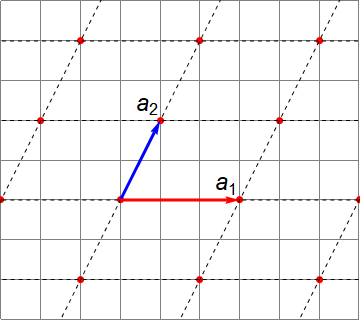
\includegraphics[width=0.40\textwidth]{HLBravaisLattice}
~~~
% (b)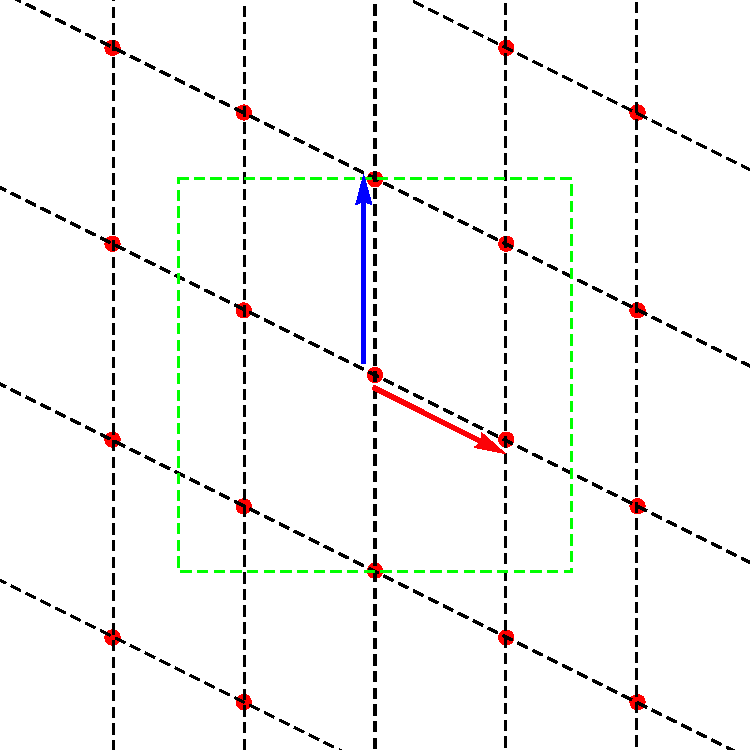
\includegraphics[width=0.40\textwidth]{HLReciprocalLattice1}
  \caption{\label{fig:BravaisLatt}
  (Color online)
%(a)
    The intersections of the (light grey) solid lines form the square
    lattice on which the discrete field $\ssp_z$ is defined. The (red)
    basis vector $\mathbf{a}_1=(3,0)$ and the (blue) basis vector
    $\mathbf{a}_2=(1,2)$ form a $\LTS{}{}{}=\BravCell{3}{2}{1}$ Bravais
    cell. The intersections (red points) of the black dashed lines form
    the Bravais lattice $\Lambda$.
        \PCedit{ %2020-09-05
    DROPPED ``\ie, the tiles on which the field \Xx\ is periodic.''
        }
% dropped \reffig{fig:HLReciprocalLattice}\'(b)
}
\end{figure}
%%%%%%%%%%%%%%%%%%%%%%%%%%%%%%%%%%%%%%%%%%%%%%%%%%%%%%%%%%%%%%%

A given Bravais \emph{lattice} $\Lambda$  can be defined by any of the infinity of
Bravais cells,
each defined by a different pair of basis vectors
$(\mathbf{a}_{1},\mathbf{a}_{2})$, but equivalent under unimodular,
\SLn{2}{\integers} transformation\rf{Lang71}.
    \PC{2020-09-05}{
recheck Lang\rf{Lang71} {\em Linear Algebra}, or replace!
It is possible that it does not reference  modular group at all...
    }
Each such family contains a unique
Bravais cell of the \emph{Hermite normal form}\rf{Cohen93}, which, for a
2\dmn\ square lattice, can be chosen to have the first basis vector
pointing in the spatial direction\rf{Lind96}
\beq
\mathbf{a}_1=\left(\begin{array}{c}
  \speriod{}\\
  0{}
  \end{array}\right)
  \,,\qquad
\mathbf{a}_2=\left(\begin{array}{c}
  \tilt{}\\
  \period{}
  \end{array}\right)
  \,,
\ee{Hermite2d}
where $\speriod{}$, $\period{}$ are respectively the spatial, temporal
lattice periods, and the `tilt'\rf{OKKH99} $0\leq\tilt{}<\speriod{}$ imposes the
relative-periodic `shift' {\bcs}\rf{ChaosBook}
(in the integer lattices literature these are also
referred to as
\emph{`helical'}\rf{LHCLL06} vs. \emph{`toroidal'}\rf{IzOgCh02};
\emph{`twisted'} and
\emph{`twisting factor'}\rf{LHCLL06};
\emph{`screw'}
{\bcs}).
We label Bravais cell \refeq{Hermite2d} and the corresponding Bravais
lattice $\Lambda$ by \LTS{}{}{}. An example is the $\BravCell{3}{2}{1}$
Bravais lattice is shown in \reffig{fig:BravaisLatt}.

\PCedit{  %2020-09-05
For each width  $\speriod{}$, height  $\period{}$,
the number of (tilted) Hermite normal form Bravais cells is
\beq
\#_{[\speriod{}\times\period{}]}
   = \sum_{\tilt{}=0}^{\speriod{}-1} 1
   = \speriod{}
\,,
\ee{noBravLatts}
and a Bravais lattices-counting zeta function (see Lind\rf{Lind96}
Example~3.1) can by constructed by substituting
$\#_{[\speriod{}\times\period{}]}$ into
\bea
1/\zeta(z)
 &=& \exp \left(-
 \sum_{\speriod{}=1}^\infty
  \sum_{\period{}=1}^\infty
  \#_{[\speriod{}\times\period{}]}
  \frac{z^{\speriod{}\period{}}}{\speriod{}\period{}}
         \right)
 =  \exp \left(-\sum_{\speriod{}=1}^\infty
                \sum_{\period{}=1}^\infty
    \frac{(z^{\speriod{}})^{\period{}}}{\period{}}
         \right)
\continue
 &=&
   \exp\left(\sum_{\speriod{}=1}^\infty
                \ln(1 - z^{\speriod{}})
         \right)
  =
\prod_{\speriod{}=1}^{\infty}(1 - z^{\speriod{}})
\,.
\label{Lind96Examp3-1}
\eea
    }
    \PC{2020-09-05}{
As long as I do not understand the logic of this zeta function,
we will have to drop it from the paper...
    }


\subsection{Prime Bravais lattices}
\label{s:primeLatt}
% PC{2020-09-05}{ This section was called ``{\em Prime \twots}'' }

It might be possible to tile a given Bravais lattice $\Lambda$
by a finer lattice $\Lambda_p$. Lattice $\Lambda_p$, defined
by a Bravais cell
\beq
\mathbf{a}^p_{1}=\left(\begin{array}{c}
  \speriod{p}\\
  0{}
  \end{array}\right)
  \,,\qquad
\mathbf{a}^p_{2}=\left(\begin{array}{c}
  \tilt{}_{p}\\
  \period{p}
  \end{array}\right)
\,,
\ee{primeTile}
is a \emph{prime} Bravais lattice, if there is no finer Bravais cell,
other than the unit volume $\BravCell{1}{1}{0}$ Bravais cell, that can
tile it.
    \PC{2020-07-15}{
   In \emph{siminos/spatiotemp/chapter/integLatt.tex} Dudgeon and
   Mersereau\rf{DudMer84} explain clearly that if $\det\Lambda$ is a
   prime number, then $\Lambda$ is a \emph{prime matrix}. If $\Lambda$ is
   neither prime nor unimodular, it is \emph{composite}, and can be
   decomposed, nonuniquely - up to a unimodular transformation - into a
   product of two non-unimodular matrices \(\Lambda=PQ\). Then one can
   ``quotient'' $Q$ by ``dividing'' by $P$.
    }

In order to determine all prime lattices $\Lambda_p$ \refeq{primeTile}
% with Bravais cells \( (\mathbf{a}^p_{1},\mathbf{a}^p_{2}) \,, \)
 that tile a given Bravais lattice $\Lambda$ \refeq{Hermite2d},
%with  Bravais cell
%\(
%(\mathbf{a}_1,\mathbf{a}_2)
%\,,
%\)
\bea
\mathbf{a}_1 &=& k\,\mathbf{a}^p_{1} + \ell\,\mathbf{a}^p_{2}
    \continue
\mathbf{a}_2 &=& m\,\mathbf{a}^p_{1} +    n\,\mathbf{a}^p_{2}
\,,
\nnu
\eea
observe that a prime tile
\(
(\mathbf{a}^p_{1},\mathbf{a}^p_{2})
\)
tiles the larger tile only if larger tile's width
$\speriod{}$ is a multiple of $\speriod{p}$, the height
$\period{}$ is a multiple of $\period{p}$, and the two tile `tilts'
satisfy
\[ %beq
\mathbf{a}_2 = {m}\,\mathbf{a}^p_{1} + \frac{\period{}}{\period{p}} \mathbf{a}^p_{2}
\quad\rightarrow\quad
\tilt{} = {m} \speriod{p} + \frac{\period{}}{\period{p}} \tilt{p}
\,.
\] %\ee{primeTiling}
Hence a prime lattice $\Lambda_p$ tiles the given lattice $\Lambda$ only if
the area spanned by the two `tilted' basis vectors
\beq
\mathbf{a}_2\times\mathbf{a}^p_{2}=\tilt{}\period{p}-\period{}\tilt{p}
\ee{primeTiling}
is a multiple of the prime tile area $\speriod{p}\period{p}$.

    \PCedit{ %2016-11-08
\subsection{Lattice states}
\label{s:lattState}

A \emph{lattice state} is a set of all field values $\Xx = \{\ssp_z\}$
over the $d$\dmn\ lattice $z\in\integers^d$ that satisfies the
\catlatt\ equation \refeq{catLatt}, with all field values constrained to
$0\leq\ssp_z<1$.

While the {\catlatt} equation \refeq{catLatt} is \emph{equivariant} under
the integer lattice \emph{space group} $p4mm$ symmetry operations
\refeq{eq:C4v}, the individual lattice states either have no symmetry at
all (they are, after all, `turbulent'), or are invariant under subgroups
of space group $p4mm$.  In what follows we quotient only the translational
symmetries, and postpone dazzling the captive reader with the full \Dn{4}
point group reduction to a later, more ponderous publication.
}

    \PCedit{ %2020-09-05
Furthermore, inspection of the \templatt\
\reffig{fig:catCycJacob} suggests that there is a \emph{field symmetry}
under inversion though the center of the $0\leq\ssp_z<1$ unit interval.
Indeed, if
$\Mm=\{\Ssym{n\zeit}\}$, composed of symbols from alphabet
\refeq{catLatt2d}, corresponds to a 2\dmn\ lattice state
${\Xx}_{\Mm}=\{\ssp_{n\zeit}\}$, its conjugation symmetry partner
\beq
\bar{\Mm}=\{\bar{\Ssym{}}_{n\zeit}\}
\,,\qquad \bar{\Ssym{}}_{n\zeit} =
2(s-2)-\Ssym{n\zeit}
\,,
\ee{Mconjug}
corresponds to lattice state
${\bar{\Xx}}_{\bar{\Mm}}=\{1-\ssp_{n\zeit}\}$. So, every lattice state
either belongs to a conjugate pair
$\{{\Xx}_{\Mm},\bar{\Xx}_{\bar{\Mm}}\}$, or is self-dual under
conjugation.
%  P 2020-09-05 tests: $2s-4-(2{s}\!-\!1)=-3$; $2s-4-(0)=2s-4 \Rightarrow 1$
}

    \PCedit{ %2020-09-05
While the action of {\jacobianOrb} $\jMorb$ \refeq{dDCatsT} maps
fields $\ssp_{n\zeit}$ to values outside the unit interval, such values
that are then returned back to the  unit interval by integer
\Ssym{n\zeit}. This `$\integers^1$ lattice action' at every \spt\ lattice site
is a peculiarity of the coupled Bernoulli and cat map lattice models, not
a condition that a \spt\ discretization of a generic field theory would
satisfy, and should never be confused with a discretization of spacetime
continuum to integer lattice $\integers^d$.
    }



    \PCedit{ %2020-09-05
For brevity, we shall refer to lattice state $\Xx$ as a
\emph{\twot} if it satisfies
\beq
\Xx({z} + {R}) = \Xx({z})
\ee{dDprimePO}
for any discrete translation
\(
{R} =n_{1}\mathbf{a}_{1}+n_{2}\mathbf{a}_{2}
\in \Lambda
\,,
\)
where $\{n_{1},n_{2}\}$ are any integers, and
$(\mathbf{a}_{1},\mathbf{a}_{2})$ is a pair of $\integers^2$ integer
lattice vectors that define a \emph{Bravais cell}. We shall always refer
to a Bravais sublattice by its unique {Hermite normal form} {Bravais
cell} \refeq{Hermite2d}, and denote it $\Lambda=\LTS{}{}{}$,
a 2\dmn\ doubly-periodic
(relative) \emph{\twot}
\beq
\ssp_{n\zeit} = \ssp_{n + \speriod{}, \zeit}
                 = \ssp_{n+\tilt{}, \zeit+ \period{}}
    \,,\qquad
(n,\zeit)\in\integers^2
\ee{Woods12p6}
with periods $(\speriod{},\period{})$ and tilt $\tilt{}$.
    }

    \PCedit{ %2020-09-05
A correct  definition of  a {\em prime} {\twot}\rf{DasBuchMirror} is
subtler than for the 1\dmn\ temporal lattice case.
If a given {\twot} over \LTS{}{}{} is not periodic under translations
\({R}\in\Lambda_p\) on any sublattice $\Lambda_p$, we shall refer to it
here as a \emph{prime {\twot}}, a \po\ of minimal periodicity in all
spacetime directions.
We return to explicit construction of prime \twots\ in \refsect{s:prime}.
Prime \twots\ are the basic building blocks of \tzeta s (see
\refsect{s:bernZeta} and \ref{s:tempCatZeta}).
    }



Explicitly verifying the periodic lattice states counting formulas for
several 2\dmn\ \catlatt\ examples is now in order.

The simplest examples of {\twots} are
(i) spacetime \eqva\ over $\BravCell{1}{1}{0}$,
(ii) space-\eqva\ over $\BravCell{1}{\period{}}{0}$,
(iii) time-\eqva\  over $\BravCell{\speriod{}}{1}{0}$,
and
(iv) time-\reqva\ over $\BravCell{\speriod{}}{1}{\tilt{}}$,  $\tilt{}\neq0$,
stationary patterns in a time-reference frame\rf{PolTor92} moving with a constant
velocity $\tilt{}/\period{}$.

\subsubsection{Spacetime \eqva\ over $\BravCell{1}{1}{0}$.}
\label{s:catLatt1x1}


\subsubsection{Time-\eqva\ over $\BravCell{\speriod{}}{1}{0}$.}
\label{s:catLattLx1}
Consider the time-\eqv\
\(
\ssp_{n\zeit} = \ssp_{n1}
\)
for all spatial sites $n$, and all times $\zeit$.
To see that this is the 1\dmn\ lattice \templatt\ tiles of period
\speriod\ already counted in \refsect{s:tempCatCount}, note that the 5-term
recurrence relation \refeq{CatMap2d} reduces to the 3-term recurrence
\beq
\ssp_{n+1,1}-2({s}_2-1)\,\ssp_{n1}+\ssp_{n-1,1}
     = -\Ssym{n1}
\,,
\ee{eq:CatLattT=1}
where we have temporarily added index `${}_2$' to the stretching parameter
${s}_2$ to indicate that it refers to the 2\dmn\ \catlatt. Comparing with
the \templatt\ \refeq{catMapNewt},
\(
\ssp_{\zeit+1}  -  {s}_1\, \ssp_{\zeit} + \ssp_{\zeit-1}
    =
-\Ssym{\zeit}
\,,
\)
we see that we have already counted all lattice states on Bravais cells of form
$\BravCell{\speriod{}}{1}{0}$, provided we replace
\(
{s}_1\to2({s}_2-1)
\)
in \refeq{1stChebGenF}. For the values chosen in
our numerical examples,
\( {s}_1=3 \)
and
\( {s}_2=5/2 \,,\)
the two counts happen to be the same and given by \refeq{catMapN_n-s=3}.

However, already the smallest \emph{relative}-periodic
\BravCell{\speriod{}}{1}{\tilt{}}
%$\BravCell{\speriod{}}{1}{0}_\tilt{}$
Bravais lattices are new, and perhaps
surprising.

\subsubsection{Relative  $\BravCell{2}{1}{1}$ \twot.}
\label{s:catLattRel2x1}

% was in siminos/spatiotemp/chapter/CL18blog.tex
% \HLpost{2019-08-08}{
Consider a $\BravCell{2}{1}{1}$ \twot\ with tilt periodic \bcs,
periodic state
\(
\Xx_{\Ssym{1}\Ssym{2}} =
 [
 \begin{array}{cc}
 \ssp_{1} & \ssp_{2}
 \end{array}
 ]
\,,
\)
tiled by the Bravais lattice
\refeq{2DBravaisLattice} with basis vectors $\mathbf{a}_1=\{2,0\}$ and $\mathbf{a}_2=\{1,1\}$, see \reffig{fig:2x1rpo}\,(a).
    \PC{2020-02-23}{
This is wrong, it is written for the symmetric alphabet that we do not use. Fix.
    }	
\beq
\Xx_{\underline{\Ssym{}}\Ssym{}} = \frac{1}{9}
 \left[
 \begin{array}{cc}
 -\Ssym{} & \Ssym{}
 \end{array}
 \right]
        \,,\qquad
\Ssym{}\in\A
         \,,
\ee{catLattRel2x1}
for example
\[
\Mm =
 \left[
 \begin{array}{cc}
 -4 & 4
 \end{array}
 \right]
 \Rightarrow\quad
\Xx_{\underline{4}4} = \frac{1}{9}
 \left[
 \begin{array}{cc}
 -4 & 4
 \end{array}
 \right]
 \,.
\]
Note that these are `periodic lattice state' solutions: there is one \emph{prime}
\twot\ for each set of period-2 periodic lattice states related by cyclic
permutations,
\(
\cycle{\underline{\Ssym{}}\Ssym{}}
    =
(\Xx_{\underline{\Ssym{}}\Ssym{}}, \Xx_{\Ssym{}\underline{\Ssym{}}})
\,,
\)
and there are only 4 of those, as $\Xx_{00}=\Xx_{0}$ is a repeat of the
1-\brick.

By \refeq{2x1_1Fourier} the number of $\BravCell{2}{1}{1}$ relative
\twots\ with the given Bravais lattice bc's is 9.
Using the Green's function method \refeq{GreenFuncCoupled} one can verify
that there are indeed 9 such \twots,
one \twot\ solution for each letter of alphabet \refeq{catLatt2d},

\subsubsection{$\BravCell{2}{1}{0}$ \twot.} %$[2\!\times\!2]$
\label{s:catLatt2cycles}
    %
    %    \HLpost{2019-08-12}{
As an illustration of the {\fundPip} \refeq{detBern0}
%\refeq{fundParallelo} counting of periodic solutions, consider \PV\
$s=3$ cat map \refeq{eq:StateSpCatMap} acting on states $\ssp_{\zeit}$
within the unit square $(\ssp_{0},\ssp_{1})\in|0,1)\times|0,1)$. In 2
time steps {\jacobianOrb} $\jMorb$ % $(\jMps^2 - \matId)$ stretches the
unit square into the {\fundPip}, with integer points within the
{\fundPip} corresponding to $N_2=5$ periodic lattice states
\refeq{catMapN_n-s=3} of period 2. These integer-valued vertices
over-count the number distinct lattice states, as already noted in the
construction of the \tzeta\ \refeq{Isola90-13a}.

%\paragraph{Symmetries.}

But the great thing about the \catlatt\ is that it is a field theory
defined on a lattice, a theory that can be solved by the well-developed
crystallographic methods: here we follow the
notation of Dresselhaus \etal\rf{Dresselhaus07}.

%    \HLpost{2019-11-22}{
To determine the {\em \admissible} \brick s,

(7)
compute $\Xx_p$ for each prime \brick\ $\Mm_p$, and eliminate every
$\Xx_p$ which contains a lattice site or sites on which the
value of the field violates the admissibility
condition $\ssp_z\in[0,1)$.

For $s=5/2$ \catlatt\
the pruning turns out to be very severe.
Only 52 of the prime
\PCedit{$\BravCell{2}{2}{0}$} % 2019-11-22 Han's was $[4\times4]$
{\brick}s are {\admissible}. As for the repeats of smaller {\brick}s,
there are 2 {\admissible} $\BravCell{1}{2}{0}$ {\brick}s repeating in time and 2
$\BravCell{2}{1}{0}$ {\brick}s repeating in space. There are 4 {\admissible}
$1/2$-shift periodic boundary $\BravCell{1}{2}{0}$ {\brick}s. And there is 1
admissible {\brick} which is a repeat of letter 0.
The total number of $\BravCell{2}{2}{0}$ of \twots\ is obtained by all cyclic
permutations of \admissible\ prime \brick s,
\bea
N_{\BravCell{2}{2}{0}} &=& 225
 \continue
    &=&       {52}\,\BravCell{2}{2}{0}
             + {2}\,\BravCell{2}{1}{0}
             + {2}\,\BravCell{1}{2}{0}
             + {4}\,\BravCell{2}{1}{1}
             + {1}\,\BravCell{1}{1}{0}
\,,
\label{[2x2]count}
\eea
summarized in \reftab{tab:LxTs=5/2}. This explicit list of \admissible\
prime \twots\ verifies the counting formula \refeq{2DCountingFormula}.
%    }

\subsubsection{$\BravCell{3}{2}{0}$ \twot.}
\label{s:catLattRel3x2}
%    \HLpost{2019-11-23}{
For $s=5/2$ \catlatt\
only 850 prime $\BravCell{3}{2}{0}$ \brick s are \admissible. There are 5
\admissible\ repeating prime $\BravCell{3}{1}{0}$ \brick s, 2 \admissible\
repeating prime $\BravCell{1}{2}{0}$ \brick s, and 1 \admissible\ \brick\ which
is a repeat of 0. The total number of \admissible\ solutions obtained by
all cyclic permutations of \admissible\ prime \brick s is:
     \beq
N_{\BravCell{3}{2}{0}} = 5120
=850\,\BravCell{3}{2}{0}+5\,\BravCell{3}{1}{0}+2\,\BravCell{1}{2}{0}+1\,\BravCell{1}{1}{0}
\,,
     \ee{[3x2]count}
summarized in \reftab{tab:LxTs=5/2}.
The count is in agreement with the counting formula \refeq{2DCountingFormula}
for the $\BravCell{3}{2}{0}$ \twots.


\subsubsection{Relative $\BravCell{3}{2}{1}$ \twot.}
\label{s:catLattRel3x2_1}
Consider the Bravais lattice of \reffig{fig:BravaisLatt}, tiled by \twot\
defined by the Bravais cell with basis vectors $\mathbf{a}_1=(3,0)$ and
$\mathbf{a}_2=(1,2)$, see \reffig{fig:2x1rpo}\,(b). There are 6 independent
field values in the repeating cell, which can be written as an
$[3\!\times\!2]$ array:
    \PC{2020-02-23}{
Where is the source code for \reffig{fig:2x1rpo}?
    }
\[
\BravCell{3}{2}{1} =
 \left[
 \begin{array}{cccc}
           & \ssp_{11} & \ssp_{21} & \ssp_{01} \\
 \ssp_{00} & \ssp_{10} & \ssp_{20} &
 \end{array}
 \right]
\,.
\]

\noindent{\em Example: $\BravCell{2}{2}{0}$ Bravais
                lattices prime {\brick}s.}
%\label{s:prime2tori2x2}

%    \HLpost{2019-11-22}{
Consider $\BravCell{2}{2}{0}$ Bravais
lattices prime {\brick}
\beq
\Mm_p=
        \left[\begin{array}{cc}
\Ssym{01} & \Ssym{11}   \\
\Ssym{00} & \Ssym{10}
              \end{array}\right]
\,,
\ee{eq:block2x2}


According to \refeq{primeCount2D}, the number of prime % primitive
$\BravCell{2}{2}{0}$ lattice states is
\bea
M_{\BravCell{2}{2}{0}}&=&\frac{1}{2\cdot2}
  \left( N_{\BravCell{2}{2}{0}}
            - 2M_{\BravCell{2}{1}{0}}
%    \right.\ceq\left.\qquad\qquad
            - 2M_{\BravCell{1}{2}{0}}
            - 2M_{\BravCell{2}{1}{1}}
            - M_{\BravCell{1}{1}{0}}
  \right)
\,,
\label{catlattM2x2}
\eea
We can work this out explicitly as follows:\\

(3) The $\BravCell{2}{1}{1}$ relative-periodic {\brick} \refeq{eq:block2x1rp} is
counted as the $\BravCell{2}{2}{0}$ \twot.

(5) Throw away all {\brick}s which are repeats of
shorter {\brick}s. There are three kinds of repeating small {\brick}s:
\[
\BravCell{2}{1}{0}=\left[\begin{array}{cc}
a & b \\
a & b \\
              \end{array}\right]
\, , \quad
\BravCell{1}{2}{0}=\left[\begin{array}{cc}
b & b \\
a & a \\
              \end{array}\right]
\, , \quad
\BravCell{2}{1}{1}=\left[\begin{array}{ccc}
  & a & b \\
a & b &   \\
              \end{array}\right]
\,.
\]


\bigskip

the relative-periodic $\BravCell{2}{1}{1}$ {\brick} with $1$ site-shift
periodic boundary, which is periodic after the second repeat in the time
direction,
\beq
\Mm_p=
        \left[\begin{array}{ccc}
           &  \left[\Ssym{00}\right.&\left.\Ssym{10}\right] \\
\left[\Ssym{00}\right.&\left.\Ssym{10}\right] &
         \end{array}\right]
\,.
\ee{eq:block2x1rp}


\noindent{\em Example: $\BravCell{3}{2}{0}$  Bravais
                lattices prime {\brick}s.}
%\label{s:prime2tori3x2}

Consider the Bravais lattice
\beq
\Mm=
        \left[\begin{array}{ccc}
\Ssym{12} & \Ssym{22} & \Ssym{32}   \\
\Ssym{11} & \Ssym{21} & \Ssym{31}
              \end{array}\right]
\,.
\ee{eq:block3x2}
According to \refeq{primeCount2D}, the number of prime %primitive
$\BravCell{3}{2}{0}$ lattice states is
\bea
M_{\BravCell{3}{2}{0}}&=&\frac{1}{3\cdot2}
  \left( N_{\BravCell{3}{2}{0}}
            - 3M_{\BravCell{3}{1}{0}}
%    \right.\ceq\left.\qquad\qquad
            - 2M_{\BravCell{1}{2}{0}}
            - M_{\BravCell{1}{1}{0}}
  \right)
\,,
\label{catlattM3x2}
\eea
Unlike the $\BravCell{2}{2}{0}$ case \refeq{eq:block2x1rp}, there no sub-\brick s
with relative-periodic boundary contributing to the $\BravCell{3}{2}{0}$ \brick s
count, since $\BravCell{3}{1}{0}$ and $\BravCell{1}{2}{0}$ sub-\brick s cannot fit into
the $\BravCell{3}{2}{0}$ doubly-periodic Bravais lattice without a shift.

\subsection{Counting \catlatt\ lattice states}
\label{s:catLattCount}

We now show how to count the number of periodic lattice states of a $2$\dmn\
\catlatt, and apply the method
to counting {\twots} of the 2\dmn\ \catlatt.

Periodic lattice {\HillDet}s, such as \refeq{detBern0}, are usually
evaluated by a Fourier transform diagonalization (see
\refappe{appe:Fourier}). However, due to the uniformity of Bernoulli map
stretching, in case at hand lattice points counting is a combinatorial
problem. Counting of $\integers^d$ integer lattice points within various
convex domains is an important, highly developed field. For integer
lattice counting powerful combinatorial methods are available, for
example Barvinok multivariate generating functions algorithm for counting
lattice points in convex lattice domains\rf{Barvinok94}, and its online
code implementations, such as the lattice point enumeration
\texttt{LattE} code\rf{DeLHTY04}.

As in the \templatt\ case \refeq{detCat0}, the total number of periodic
lattice states is given by the volume of the {\fundPip}
\beq
N_\cl{} = |\Det\jMorb|
\,.
\ee{detCatlatt}

\subsection{Stability of an orbit vs. its time-evolution stability}
\label{s:catLattHill}

\subsection{\Po\ theory}
\label{s:catLattPoThe}

    \PC{2020-02-02}{
Gutkin and Osipov\rf{GutOsi15} refer to an \sPe\ \twot\ solution $p$ as a
`many-particle periodic orbit', with $\ssp_{n\zeit}$ `doubly-periodic',
or `closed,'
\[
\ssp_{n\zeit} = \ssp_{n+\speriod{p},\zeit+\period{p}}
    \,,\quad
n = 0,1,2,\cdots, \speriod{p}-1
    \,;\quad
\zeit = 0,1,2,\cdots, \period{p}-1
    \,.
\]
    }


\subsection{Shadowing}
\label{s:catLattShadow}

    \PC{2019-08-06}{
Must emphasize {\em shadowing}? One of the main points of this and the
companion papers is that \po s shadowing generalizes to \twots\ shadowing
in higher \spt\ dimensions. Include 2d \twots\ shadowing figures.

Add a shadowing sub-section here, the analogue to
\templatt\ Green's function \refeq{1dLatGreenFct}.
    }


As we now show, the
{\brick}
\(
\Mm= \{\Ssym{nt} \in \A \,,\; (n,t)\in \integers^2 \}
\)
can be used as a 2\dmn\ symbolic representation of the lattice system
state.
By the linearity of equation \refeq{2dCoupledCats}, every solution \Xx\
can be uniquely recovered from its symbolic representation \Mm. Inverting
\refeq{2dCoupledCats} we obtain
\beq
  \ssp_{z}=\sum_{z'\in\integers^2}g_{z z'} \Ssym{z'}, \qquad  g_{z z' }
       =\left(\frac{1}{-\Box +2(s -2)}\right)_{zz'}
       \,,
\ee{GreenFuncCoupled}
where  $g_{z z'}$
% $z=(n,t)\in\Zz$,  $z'=(n',t')\in\Zz$,
is the  Green's
function for the 2\dmn\ discretized \sPe.
However, a given lattice \brick\ $\Mm$ %=\{\Ssym{z}|z\in\Zz\}$
is \emph{{\admissible}} if and only if all  $\ssp_{z}\in \Xx$ given by
\refeq{GreenFuncCoupled} fall into the interval $[0,1)$.

For a given
admissible source \brick\ $\Mm$, the periodic field can be computed by:
\[
\Xx_{i_1 j_1} =
\sum_{i_2=0}^2 \sum_{j_2=0}^1 \gd_{i_1 j_1,i_2 j_2} \Mm_{i_2 j_2} \, .
\]
For example, if the source $\Mm$ is:
\[
\Mm =
 \left[
 \begin{array}{ccc}
 0 & 2 & 0 \\
 -1 & 0 & 0
 \end{array}
 \right] \, ,
\]
the corresponding field is:
\[
\Xx_\Mm =
 \left[
 \begin{array}{ccc}
 \ssp_{01} & \ssp_{11} & \ssp_{21} \\
 \ssp_{00} & \ssp_{10} & \ssp_{20}
 \end{array}
 \right]
 =
 \frac{1}{35}
 \left[
 \begin{array}{ccc}
 5 & 17 & 6 \\
 -1 & 5 & 3
 \end{array}
 \right] \, .
\]
Substitute this solution into \reffig{fig:2x1rpo}\,(b) we
can see that \refeq{CatMap2d} is satisfied everywhere.

\subsection{{\Tzeta}}
\label{s:catLattZeta}

\subsection{\tempLatt\ as a continuous time dynamical system}
\label{s:catLattODE}

\beq
 (\Box -2(s-2))\,\Xx = -\Mm
\ee{LinearCatLatt}

While the $d=2$ \catlatt\ does have a Hamiltonian
formulation\rf{GutOsi15}, its Lagrangian  formulation as {\sPe}
\refeq{LinearCatLatt}, in analogy with the {\templatt} \refeq{OneCat}, is
a natural departure point for what follows:
\bea
 (\Box -2({s}-2))\,\ssp_{n\zeit} &=& -\Ssym{n\zeit}
    \,, \qquad
  \ssp_{n\zeit} \in [0,1)
    \,, \quad
  \Ssym{n\zeit} \in \A
    \,, \quad
  (n,\zeit)\in \integers^{2}
\,,
\label{2dCoupledCats}
\eea
where $\Box$ is now the discrete 2\dmn\ space-time Laplacian
on $\integers^2$,
\beq
\Box\,\ssp_{n\zeit} =                   \ssp_{n,t-1} + \ssp_{n-1,t}
                   - 4\,\ssp_{n\zeit} + \ssp_{n,t+1} + \ssp_{n+1,t}
\,,
\ee{2dLaplSpaceTime}
and the alphabet is given in \refeq{catLatt2d}.

    \PC{2019-01-04} {
More generally, the same argument yields the {\sPe} \refeq{OneCat} for
the $d$\dmn\ {\em \catlatt}
\bea
 (\Box - d({s}-2))\,\ssp_{z} &=& -\Ssym{z}
    \,, \qquad
  \ssp_{z} \in [0,1)
    \,, \quad
  \Ssym{z} \in \A
    \,, \quad
  z\in \integers^{d}
\,,
\continue
 && \A = \{-2d+1, -2d+2,\cdots,2{s}-2,2{s}-1\}
\,,
\label{LinearConn}
\eea
where $\Box$ is the discrete $d$\dmn\ Euclidean space-time Laplacian.
}

    \PC{2019-01-04} {

The $d$\dmn\ \catlatt\ satisfies {\sPe} \refeq{dDCatsT}
\beq
(\Box -d(s - 2))\,\ssp_{z} =-\Ssym{z}
\,,\qquad
{z} \in \integers^d
\,,
\ee{dDCats}
where $\Box$ is the discrete $d$\dmn\ Laplacian
(discrete Laplacians on 1\dmn\ and 2\dmn\ lattices are given in
\refeq{PerViv2.2} and \refeq{2dLaplSpaceTime}). As in \refeq{action}, a
$d$\dmn\ discrete Laplacian can be written as
\beq
\Box = \sum_{i=1}^{d} (\hopMat_{i}  - 2\unit + \hopMat_{i}^{-1})
\,,
\ee{dDLapl}
    }


------------------------------------------------------

\bigskip

\noindent\textbf{\catLatt, summarized.}
The
key insight\rf{BunSin88,GutOsi15} --an insight that applies to coupled-map
lattices\rf{PolTor92b,PetCorBol06,PetCorBol07}, and field theories
modeled by them, not only the system considered here-- is that a field
\(
\Xx=\{\ssp_{z}\} % = \{\ssp_{z},  z\in \integers^{d}  \}
\)
over a $d$\dmn\ spacetime lattice $z\in \integers^{d}$ has to be
described by a corresponding symbol {\brick}
\(
\Mm=\{\m_{z}\} % = \{\m_{z}, z\in \integers^{d}\}
\,,
\)
over the same $d$\dmn\ spacetime  lattice $z\in \integers^{d}$, rather
than a 1\dmn\ temporal symbol sequence \refeq{linCode}, as one does when
describing a finite coupled ``$N$-particle'' system in the Hamiltonian
formalism.

A key advantage of the {\spt} code \Mm\ is illustrated already by the $d=2$
case. While an \AW\ type partition, forward-in time Hamiltonian evolution
alphabet would grow exponentially with the
``particle number'' $\speriod{}$, the number of letters
\refeq{dDCatsT} of the {\spt} code \A\ is finite and the same for any
spatial extent
$\speriod{}$, including the $\speriod{}\to\infty$ \catlatt. For the
{\spt} code, a field \Xx\ over a periodic \spt\ domain is encoded by a
doubly periodic 2\dmn\ {\brick} $\Mm$ of symbols from a small alphabet,
rather then by a $1$\dmn\ temporal string of symbols from the
exponentially large (in $\speriod{}$) `\speriod{}-particle' alphabet
\Aa.

The
{\catlatt} is arguably the simplest example of a chaotic (or `turbulent')
classical field theory for which the local degrees of freedom are
hyperbolic (anti-harmonic, `inverted pendula') rather than oscillatory
(`harmonic oscillators'). As we have shown here, it is also a field theory
for which all {\admissible} {\spt} patterns can be enumerated, and their
recurrences (shadowing of a large \twot\ by smaller \twots) identified.
